%%%  کلاس AUTthesis، نسخه آبان 1397
%%%   دانشگاه صنعتی امیرکبیر                 http://www.aut.ac.ir
%%%  تالار گفتگوی پارسی‌لاتک،       http://forum.parsilatex.com
%%%   آپدیت شده در آبان 95
%%%   پشتیبانی و راهنمایی          badali_farhad@yahoo.com
%%%
%%%   بازبینی و اصلاح شده در آبان ماه 1397
%%%  Tested via TeXstudio in TeXlive 2014-2018.
%%%

%-----------------------------------------------------------------------------------------------------
%        روش اجرا.: 2 بار F1 ، 2 بار  F11(به منظور تولید مراجع) ، دوبار Ctrl+Alt+I (به منظور تولید نمایه) و دو بار F1 -------> مشاهده Pdf
%%%%%%%%%%%%%%%%%%%%%%%%%%%%%%%%%%%%%%%%%%%%%%%%%%%%%%
%   TeXstudio as your IDE
%%  برای compile در TeXstudio تنها کافی است منوی Options->Configure TeXstudio را زده و در پنجره Configure TeXstudio در بخش Build گزینه Default Compiler را به XeLaTeX تغییر دهید. سند شما به راحتی compile خواهد شد.
%   F1 & F5 : Build & view
%   F6      : Compile
%   F7      : View
%   --------------
%%%%%%%%%%%%%%%%%%%%%%%%%%%%%%%%%%%%%%%%%%%%%%%%%%%%%%
%        اگر قصد نوشتن رساله دکتری را دارید، در خط زیر به جای msc،
%      کلمه phd را قرار دهید. کلیه تنظیمات لازم، به طور خودکار، اعمال می‌شود.
%%% !TEX TS-program = XeLaTeX
\documentclass[oneside,bsc,12pt]{AUTthesis}
%       فایل commands.tex را حتماً به دقت مطالعه کنید؛ چون دستورات مربوط به فراخوانی بسته زی‌پرشین 
%       و دیگر بسته‌ها و ... در این فایل قرار دارد و بهتر است که با نحوه استفاده از آنها آشنا شوید. توجه شود برای نسخه نهایی پایان‌نامه حتماً hyperref را 
%        غیرفعال کنید.


\usepackage{booktabs}

% در این فایل، دستورها و تنظیمات مورد نیاز، آورده شده است.
%-------------------------------------------------------------------------------------------------------------------
% در ورژن جدید زی‌پرشین برای تایپ متن‌های ریاضی، این سه بسته، حتماً باید فراخوانی شود.
\usepackage{amsthm,amssymb,amsmath,amsfonts}
% بسته‌ای برای تنطیم حاشیه‌های بالا، پایین، چپ و راست صفحه
\usepackage[top=30mm, bottom=30mm, left=25mm, right=30mm]{geometry}
% بسته‌‌ای برای ظاهر شدن شکل‌ها و تصاویر متن
\usepackage{graphicx}
\usepackage{color}
%بسته‌ای برای تنظیم فاصله عمودی خط‌های متن
\usepackage{setspace}
\usepackage{titletoc}
\usepackage{tocloft}
%با فعال کردن بسته زیر فوت‌نوت‌ها در هر صفحه ریست می‌شوند. حالت پیش‌فرض آن ریست شدن در هر فصل می‌باشد.
%\usepackage[perpage]{footmisc}
\usepackage{enumitem}
%\usepackage{titlesec}
% بسته‌ و دستوراتی برای ایجاد لینک‌های رنگی با امکان جهش

%\usepackage[pagebackref=false,colorlinks,linkcolor=blue,citecolor=red]{hyperref}
\usepackage[pagebackref=false,colorlinks,linkcolor=black,citecolor=black]{hyperref}
\usepackage[nameinlink]{cleveref}%capitalize,,noabbrev
 \AtBeginDocument{%
    \crefname{equation}{برابری}{equations}%
    \crefname{chapter}{فصل}{chapters}%
    \crefname{section}{بخش}{sections}%
    \crefname{appendix}{پیوست}{appendices}%
    \crefname{enumi}{مورد}{items}%
    \crefname{footnote}{زیرنویس}{footnotes}%
    \crefname{figure}{شکل}{figures}%
    \crefname{table}{جدول}{tables}%
    \crefname{theorem}{قضیه}{theorems}%
    \crefname{lemma}{لم}{lemmas}%
    \crefname{corollary}{نتیجه}{corollaries}%
    \crefname{proposition}{گزاره}{propositions}%
    \crefname{definition}{تعریف}{definitions}%
    \crefname{result}{نتیجه}{results}%
    \crefname{example}{مثال}{examples}%
    \crefname{remark}{نکته}{remarks}%
    \crefname{note}{یادداشت}{notes}%
}
% چنانچه قصد پرینت گرفتن نوشته خود را دارید، خط بالا را غیرفعال و  از دستور زیر استفاده کنید چون در صورت استفاده از دستور زیر‌‌، 
% لینک‌ها به رنگ سیاه ظاهر خواهند شد که برای پرینت گرفتن، مناسب‌تر است
%\usepackage[pagebackref=false]{hyperref}
% بسته‌ لازم برای تنظیم سربرگ‌ها
\usepackage{fancyhdr}
% بسته‌ای برای ظاهر شدن «مراجع»  در فهرست مطالب
\usepackage[nottoc]{tocbibind}
% دستورات مربوط به ایجاد نمایه
\usepackage{makeidx,multicol}
\setlength{\columnsep}{1.5cm}

%%%%%%%%%%%%%%%%%%%%%%%%%%
\usepackage{verbatim}
\makeindex
\usepackage{sectsty}
% فراخوانی بسته زی‌پرشین و تعریف قلم فارسی و انگلیسی
\usepackage{xepersian}%[extrafootnotefeatures]
\SepMark{-}
%حتماً از تک لایو 2014 استفاده کنید.
\settextfont[Scale=1.2]{B Nazanin}
\setlatintextfont{Times New Roman}
\renewcommand{\labelitemi}{$\bullet$}
%%%%%%%%%%%%%%%%%%%%%%%%%%
% چنانچه می‌خواهید اعداد در فرمول‌ها، انگلیسی باشد، خط زیر را غیرفعال کنید.
%در غیر اینصورت حتماً فونت PGaramond را نصب کنید.
%\setdigitfont[Scale=1.1]{PGaramond}%%Yas
%%%%%%%%%%%%%%%%%%%%%%%%%%
% تعریف قلم‌های فارسی اضافی برای استفاده در بعضی از قسمت‌های متن
\defpersianfont\nastaliq[Scale=2]{IranNastaliq}
\defpersianfont\chapternumber[Scale=3]{B Nazanin}
%\chapterfont{\centering}%
%%%%%%%%%%%%%%%%%%%%%%%%%%
% دستوری برای تغییر نام کلمه «اثبات» به «برهان»
\renewcommand\proofname{\textbf{برهان}}

% دستوری برای تغییر نام کلمه «کتاب‌نامه» به «منابع و مراجع«
\renewcommand{\bibname}{منابع و مراجع}


% Headings for every page of ToC, LoF and Lot
\setlength{\cftbeforetoctitleskip}{-1.2em}
\setlength{\cftbeforelottitleskip}{-1.2em}
\setlength{\cftbeforeloftitleskip}{-1.2em}
\setlength{\cftaftertoctitleskip}{-1em}
\setlength{\cftafterlottitleskip}{-1em}
\setlength{\cftafterloftitleskip}{-1em}
%%\makeatletter
%%%%\renewcommand{\l@chapter}{\@dottedtocline{1}{1em\bfseries}{1em}}
%%%%\renewcommand{\l@section}{\@dottedtocline{2}{2em}{2em}}
%%%%\renewcommand{\l@subsection}{\@dottedtocline{3}{3em}{3em}}
%%%%\renewcommand{\l@subsubsection}{\@dottedtocline{4}{4em}{4em}}
%%%%\makeatother


\newcommand\tocheading{\par عنوان\hfill صفحه \par}
\newcommand\lofheading{\hspace*{.5cm}\figurename\hfill صفحه \par}
\newcommand\lotheading{\hspace*{.5cm}\tablename\hfill صفحه \par}

\renewcommand{\cftchapleader}{\cftdotfill{\cftdotsep}}
\renewcommand{\cfttoctitlefont}{\hspace*{\fill}\LARGE\bfseries}%\Large
\renewcommand{\cftaftertoctitle}{\hspace*{\fill}}
\renewcommand{\cftlottitlefont}{\hspace*{\fill}\LARGE\bfseries}%\Large
\renewcommand{\cftafterlottitle}{\hspace*{\fill}}
\renewcommand{\cftloftitlefont}{\hspace*{\fill}\LARGE\bfseries}
\renewcommand{\cftafterloftitle}{\hspace*{\fill}}

%%%%%%%%%%%%%%%%%%%%%%%%%%
% تعریف و نحوه ظاهر شدن عنوان قضیه‌ها، تعریف‌ها، مثال‌ها و ...
%برای شماره گذاری سه تایی قضیه ها
\theoremstyle{definition}
\newtheorem{definition}{تعریف}[section]
\newtheorem{remark}[definition]{نکته}
\newtheorem{note}[definition]{یادداشت}
\newtheorem{example}[definition]{نمونه}
\newtheorem{question}[definition]{سوال}
\newtheorem{remember}[definition]{یاداوری}
\theoremstyle{theorem}
\newtheorem{theorem}[definition]{قضیه}
\newtheorem{lemma}[definition]{لم}
\newtheorem{proposition}[definition]{گزاره}
\newtheorem{corollary}[definition]{نتیجه}
%%%%%%%%%%%%%%%%%%%%%%%%
%%%%%%%%%%%%%%%%%%%
%%% برای شماره گذاری چهارتایی قضیه ها و ...
%%\newtheorem{definition1}[subsubsection]{تعریف}
%%\newtheorem{theorem1}[subsubsection]{قضیه}
%%\newtheorem{lemma1}[subsubsection]{لم}
%%\newtheorem{proposition1}[subsubsection]{گزاره}
%%\newtheorem{corollary1}[subsubsection]{نتیجه}
%%\newtheorem{remark1}[subsubsection]{نکته}
%%\newtheorem{example1}[subsubsection]{مثال}
%%\newtheorem{question1}[subsubsection]{سوال}

%%%%%%%%%%%%%%%%%%%%%%%%%%%%

% دستورهایی برای سفارشی کردن صفحات اول فصل‌ها
\makeatletter
\newcommand\mycustomraggedright{%
 \if@RTL\raggedleft%
 \else\raggedright%
 \fi}
\def\@makechapterhead#1{%
\thispagestyle{style1}
\vspace*{20\p@}%
{\parindent \z@ \mycustomraggedright
\ifnum \c@secnumdepth >\m@ne
\if@mainmatter

\bfseries{\Huge \@chapapp}\small\space {\chapternumber\thechapter}
\par\nobreak
\vskip 0\p@
\fi
\fi
\interlinepenalty\@M 
\Huge \bfseries #1\par\nobreak
\vskip 120\p@

}

%\thispagestyle{empty}
\newpage}
\bidi@patchcmd{\@makechapterhead}{\thechapter}{\tartibi{chapter}}{}{}
\bidi@patchcmd{\chaptermark}{\thechapter}{\tartibi{chapter}}{}{}
\makeatother

\pagestyle{fancy}
\renewcommand{\chaptermark}[1]{\markboth{\chaptername~\tartibi{chapter}: #1}{}}

\fancypagestyle{style1}{
\fancyhf{} 
\fancyfoot[c]{\thepage}
\fancyhead[R]{\leftmark}%
\renewcommand{\headrulewidth}{1.2pt}
}


\fancypagestyle{style2}{
\fancyhf{}
\fancyhead[R]{چکیده}
\fancyfoot[C]{\thepage{}}
\renewcommand{\headrulewidth}{1.2pt}
}

\fancypagestyle{style3}{%
  \fancyhf{}%
  \fancyhead[R]{فهرست نمادها}
  \fancyfoot[C]{\thepage}%
  \renewcommand{\headrulewidth}{1.2pt}%
}

\fancypagestyle{style4}{%
  \fancyhf{}%
  \fancyhead[R]{فهرست جداول}
  \fancyfoot[C]{\thepage}%
  \renewcommand{\headrulewidth}{1.2pt}%
}

\fancypagestyle{style5}{%
  \fancyhf{}%
  \fancyhead[R]{فهرست اشکال}
  \fancyfoot[C]{\thepage}%
  \renewcommand{\headrulewidth}{1.2pt}%
}

\fancypagestyle{style6}{%
  \fancyhf{}%
  \fancyhead[R]{فهرست مطالب}
  \fancyfoot[C]{\thepage}%
  \renewcommand{\headrulewidth}{1.2pt}%
}

\fancypagestyle{style7}{%
  \fancyhf{}%
  \fancyhead[R]{نمایه}
  \fancyfoot[C]{\thepage}%
  \renewcommand{\headrulewidth}{1.2pt}%
}

\fancypagestyle{style8}{%
  \fancyhf{}%
  \fancyhead[R]{منابع و مراجع}
  \fancyfoot[C]{\thepage}%
  \renewcommand{\headrulewidth}{1.2pt}%
}
\fancypagestyle{style9}{%
  \fancyhf{}%
  \fancyhead[R]{واژه‌نامه‌ی فارسی به انگلیسی}
  \fancyfoot[C]{\thepage}%
  \renewcommand{\headrulewidth}{1.2pt}%
}
%


%دستور حذف نام لیست تصاویر و لیست جداول از فهرست مطالب
\newcommand*{\BeginNoToc}{%
  \addtocontents{toc}{%
    \edef\protect\SavedTocDepth{\protect\the\protect\value{tocdepth}}%
  }%
  \addtocontents{toc}{%
    \protect\setcounter{tocdepth}{-10}%
  }%
}
\newcommand*{\EndNoToc}{%
  \addtocontents{toc}{%
    \protect\setcounter{tocdepth}{\protect\SavedTocDepth}%
  }%
}
\newcounter{savepage}
\renewcommand{\listfigurename}{فهرست اشکال}
\renewcommand{\listtablename}{فهرست جداول}
%\renewcommand\cftsecleader{\cftdotfill{\cftdotsep}}
%%%%%%%%%%%%%%%%%%%%%%%%%%%%%
%%%%%%%%%%%%%%%%%%%%%%%%%%%%

\begin{document}
\baselineskip=.75cm
\linespread{1.75}
%\baselineskip=1.75cm
%\linespread{1.75}
%% -!TEX root = AUTthesis.tex
% در این فایل، عنوان پایان‌نامه، مشخصات خود، متن تقدیمی‌، ستایش، سپاس‌گزاری و چکیده پایان‌نامه را به فارسی، وارد کنید.
% توجه داشته باشید که جدول حاوی مشخصات پروژه/پایان‌نامه/رساله و همچنین، مشخصات داخل آن، به طور خودکار، درج می‌شود.
%%%%%%%%%%%%%%%%%%%%%%%%%%%%%%%%%%%%
% دانشکده، آموزشکده و یا پژوهشکده  خود را وارد کنید
\faculty{دانشکده مهندسی کامپیوتر}
% گرایش و گروه آموزشی خود را وارد کنید
\department{}
% عنوان پایان‌نامه را وارد کنید
\fatitle{طبقه بندی ترافیک شبکه 
\\[.75 cm]
 با استفاده از الگوریتم‌های یادگیری ماشین}
% نام استاد(ان) راهنما را وارد کنید
\firstsupervisor{دکتر رضا صفابخش}
%\secondsupervisor{استاد راهنمای دوم}
% نام استاد(دان) مشاور را وارد کنید. چنانچه استاد مشاور ندارید، دستور پایین را غیرفعال کنید.
%\firstadvisor{نام کامل استاد مشاور}
%\secondadvisor{استاد مشاور دوم}
% نام نویسنده را وارد کنید
\name{ محمدمهدی}
% نام خانوادگی نویسنده را وارد کنید
\surname{ هجرتی}
%%%%%%%%%%%%%%%%%%%%%%%%%%%%%%%%%%
\thesisdate{اردیبهشت 1400}

% چکیده پایان‌نامه را وارد کنید
\fa-abstract{
امروزه با توجه به استفاده‌ی روزافزون از شبکه‌ی اینترنت در دنیا، افزایش سریع تعداد کاربران و ظهور
برنامه‌های کاربردی تحت شبکه، ترافیک اینترنت به شدت در حال افزایش است. در نتیجه شناسایی
برنامه‌ها در شبکه، به امر پیچیده‌ای تبدیل شده است. از طرفی طبقه‌بندی جریان‌ها نقش مهمی در
امنیت و مدیریت شبکه و به‌ویژه برای مقابله با حملات دارد.
در گذشته از روش‌های گوناگونی برای طبقه‌بندی ترافیک اینترنت از جمله روش‌های مبتنی بر درگاه، یا
بررسی پیلود بسته‌ها استفاده می‌شد. اما امروزه با توجه به مشکلات و محدودیت‌های موجود در 
روش‌های قبل مثل اختصاص دادن درگاه به صورت پویا، وجود داده های رمزگذاری شده و ... ناگزیر مجبور
به استفاده از روش‌های جدید مثل یادگیری ماشین شده‌ایم.
روش‌ها و الگوریتم‌های متعددی با استفاده از یادگیری ماشین برای طبقه‌بندی ترافیک شبکه پیشنهاد
شده‌است. هدف این پژوهش بررسی این روش‌ها و ارزیابی و مقایسه‌ی روش‌های پیشنهادی موجود
می‌باشد.
}


% کلمات کلیدی پایان‌نامه را وارد کنید
\keywords{ترافیک شبکه، یادگیری ماشین، طبقه‌بندی، دسته‌بندی}



\AUTtitle
%%%%%%%%%%%%%%%%%%%%%%%%%%%%%%%%%%
%\vspace*{7cm}
%\thispagestyle{empty}
%\begin{center}
%
\includegraphics[height=5cm,width=12cm]{besm}
%\end{center}
\shipout\null
%% -!TEX root = AUTthesis.tex
% در این فایل، عنوان پایان‌نامه، مشخصات خود، متن تقدیمی‌، ستایش، سپاس‌گزاری و چکیده پایان‌نامه را به فارسی، وارد کنید.
% توجه داشته باشید که جدول حاوی مشخصات پروژه/پایان‌نامه/رساله و همچنین، مشخصات داخل آن، به طور خودکار، درج می‌شود.
%%%%%%%%%%%%%%%%%%%%%%%%%%%%%%%%%%%%
% دانشکده، آموزشکده و یا پژوهشکده  خود را وارد کنید
\faculty{دانشکده مهندسی کامپیوتر}
% گرایش و گروه آموزشی خود را وارد کنید
\department{}
% عنوان پایان‌نامه را وارد کنید
\fatitle{طبقه بندی ترافیک شبکه 
\\[.75 cm]
 با استفاده از الگوریتم‌های یادگیری ماشین}
% نام استاد(ان) راهنما را وارد کنید
\firstsupervisor{دکتر رضا صفابخش}
%\secondsupervisor{استاد راهنمای دوم}
% نام استاد(دان) مشاور را وارد کنید. چنانچه استاد مشاور ندارید، دستور پایین را غیرفعال کنید.
%\firstadvisor{نام کامل استاد مشاور}
%\secondadvisor{استاد مشاور دوم}
% نام نویسنده را وارد کنید
\name{ محمدمهدی}
% نام خانوادگی نویسنده را وارد کنید
\surname{ هجرتی}
%%%%%%%%%%%%%%%%%%%%%%%%%%%%%%%%%%
\thesisdate{اردیبهشت 1400}

% چکیده پایان‌نامه را وارد کنید
\fa-abstract{
امروزه با توجه به استفاده‌ی روزافزون از شبکه‌ی اینترنت در دنیا، افزایش سریع تعداد کاربران و ظهور
برنامه‌های کاربردی تحت شبکه، ترافیک اینترنت به شدت در حال افزایش است. در نتیجه شناسایی
برنامه‌ها در شبکه، به امر پیچیده‌ای تبدیل شده است. از طرفی طبقه‌بندی جریان‌ها نقش مهمی در
امنیت و مدیریت شبکه و به‌ویژه برای مقابله با حملات دارد.
در گذشته از روش‌های گوناگونی برای طبقه‌بندی ترافیک اینترنت از جمله روش‌های مبتنی بر درگاه، یا
بررسی پیلود بسته‌ها استفاده می‌شد. اما امروزه با توجه به مشکلات و محدودیت‌های موجود در 
روش‌های قبل مثل اختصاص دادن درگاه به صورت پویا، وجود داده های رمزگذاری شده و ... ناگزیر مجبور
به استفاده از روش‌های جدید مثل یادگیری ماشین شده‌ایم.
روش‌ها و الگوریتم‌های متعددی با استفاده از یادگیری ماشین برای طبقه‌بندی ترافیک شبکه پیشنهاد
شده‌است. هدف این پژوهش بررسی این روش‌ها و ارزیابی و مقایسه‌ی روش‌های پیشنهادی موجود
می‌باشد.
}


% کلمات کلیدی پایان‌نامه را وارد کنید
\keywords{ترافیک شبکه، یادگیری ماشین، طبقه‌بندی، دسته‌بندی}



\AUTtitle
%%%%%%%%%%%%%%%%%%%%%%%%%%%%%%%%%%
%\vspace*{7cm}
%\thispagestyle{empty}
%\begin{center}
%
\includegraphics[height=5cm,width=12cm]{besm}
%\end{center}
% تاییدیه دفاع
%\newpage
\thispagestyle{empty}
%\fontsize{18pt}{19pt}\selectfont

\section*{صفحه فرم ارزیابی و تصویب پایان نامه- فرم تأیید اعضاء كميته دفاع}

\fontsize{12pt}{14pt}\selectfont
%\renewcommand{\baselinestretch}{1.5}
\vspace*{1cm}
   در این صفحه فرم دفاع یا تایید و تصویب پایان نامه موسوم به فرم کمیته دفاع- موجود در پرونده آموزشی- را قرار دهید.
\vspace*{1cm}


\subsection*{نکات مهم:}
 
\begin{itemize}
\item
	نگارش پایان نامه/رساله باید به
	{\color{red}
		زبان فارسی
	}
	و بر اساس آخرین نسخه دستورالعمل و راهنمای تدوین پایان نامه های دانشگاه صنعتی امیرکبیر باشد.(دستورالعمل و راهنمای حاضر)
\item رنگ جلد پایان نامه/رساله چاپي كارشناسي، كارشناسي ارشد و دكترا  بايد به ترتيب مشكي، طوسي و سفيد رنگ باشد.  
\item چاپ و صحافی پایان نامه/رساله بصورت
{\color{red}
	پشت و رو(دورو)
}
بلامانع است و انجام آن توصيه مي شود. 
\end{itemize}
%%%%%%%%%%%%%%%%%%%%%%%%%%%%%%%%%%%%%%%%%%%%%%%%%%%%%%%%%%%%%%%%%%%%%%%%%%%%%%%%%%%%%%%%%%%%%%%%%%
%%%%%%%%%%%%%%%%%%%%%%%%%%%%%%%%%%%%%%%%%%%%%%%%%%%%%%%%%%%%%%%%%%%%%%%%%%%%%%%%%%%%%%%%%%%%%%%%%%
\newpage
\thispagestyle{empty}
\begin{picture}(50,50)
  \put(17,0){
\includegraphics[scale=1.1]{fa-logo}}
  \put(4.5,-13){\footnotesize{دانشگاه صنعتی امیرکبیر}}
  \put(10.5,-27){\footnotesize{(پلی‌تکنیک تهران)}}
  \put(170,30){\bf{به نام خدا}}
  \put(140,-5){\Large\bf{تعهدنامه اصالت اثر}}
  \put(310,0){تاریخ: \datethesis}
\end{picture}

\vspace*{2.5cm}

اينجانب {\bf{\fname\lname}} متعهد می‌شوم که مطالب مندرج در این پایان‌نامه حاصل کار پژوهشی اینجانب تحت نظارت و راهنمایی اساتید دانشگاه صنعتی امیرکبیر بوده و به دستاوردهای دیگران که در این پژوهش از آنها استفاده شده است مطابق مقررات و روال متعارف ارجاع و در فهرست منابع و مآخذ ذکر گردیده است. این پایان‌نامه قبلاً برای احراز هیچ مدرک هم‌سطح یا بالاتر ارائه نگردیده است.

در صورت اثبات تخلف در هر زمان، مدرک تحصیلی صادر شده توسط دانشگاه از درجه اعتبار ساقط بوده و دانشگاه حق پیگیری قانونی خواهد داشت.


کلیه نتایج و حقوق حاصل از این پایان‌نامه متعلق به دانشگاه صنعتی امیرکبیر می‌باشد. هرگونه استفاده از نتایج علمی و عملی، واگذاری اطلاعات به دیگران یا چاپ و تکثیر، نسخه‌برداری، ترجمه و اقتباس از این پایان نامه بدون موافقت کتبی دانشگاه صنعتی امیرکبیر ممنوع است. 
نقل مطالب با ذکر مآخذ بلامانع است.\\
\vspace{2.5cm}


{\centerline {\bf{\fname\lname}}}
\vspace*{.2cm}
{\centerline{امضا}}
%%%%%%%%%%%%%%%%%%%%%%%%%%%%%%%%%
\fontsize{12pt}{14pt}\selectfont
% چنانچه مایل به چاپ صفحات «تقدیم»، «نیایش» و «سپاس‌گزاری» در خروجی نیستید، خط‌های زیر را با گذاشتن ٪  در ابتدای آنها غیرفعال کنید.
% پایان‌نامه خود را تقدیم کنید
% نیایش خود را در فایل زیر بنویسید.
%\begin{acknowledgementpage}

\vspace{1.5cm}

{\nastaliq
{
 نويسنده پايان‌نامه، درصورت تمايل ميتواند برای سپاسگزاری پايان‌نامه خود را به شخص يا اشخاص و يا ارگان خاصی تقدیم نماید.
}}\end{acknowledgementpage}
\newpage
% سپاسگزاری را در فایل زیر بنویسید.
%%%%%%%%%%%%%%%%%%%%%%%%%%%%%%%%%%%%
\newpage\thispagestyle{empty}
% سپاس‌گزاری
{\nastaliq
سپاس‌گزاری
}
\\[2cm]

 بی‌تردید تهیه‌ی این گزارش بدون راهنمایی‌های ارزشمند استاد بزرگوار جناب آقای دکتر رضا صفابخش میسر نمی شد. بدین وسیله بر خود لازم می‌دانم از زحمات بی‌دریغ ایشان صمیمانه تقدیر و تشکر نمایم. 














% با استفاده از دستور زیر، امضای شما، به طور خودکار، درج می‌شود.
\signature








%%%%%%%%%%%%%%%%%%%%%%%%%%%%%%%%%%%%%%%%%
%%%%%%%%%%%%%%%%%%%%%%%%%%%%%%%%%کدهای زیر را تغییر ندهید.
\newpage\clearpage

\pagestyle{style2}

\vspace*{-1cm}
\section*{\centering چکیده}
%\addcontentsline{toc}{chapter}{چکیده}
\vspace*{.5cm}
\ffa-abstract
\vspace*{2cm}


{\noindent\large\textbf{واژه‌های کلیدی:}}\par
\vspace*{.5cm}
\fkeywords
% دستور زیر برای شماره گذاری صفحات قبل از فصل اول با حروف ابجد است.
\pagenumbering{alph}
%-----------------------------------------------------------------------------
% فایل زیر دستورات مربوط به نمایش صفحات فهرست مطالب- فهرست اشکال و جداول است.
%{\pagestyle{style2}
%\tableofcontents}\newpage
%
%\listoffigures
\cleardoublepage
\pagestyle{style6}
\tableofcontents
\pagestyle{style6}
\cleardoublepage
%اگر لیست تصاویر و لیست جداول ندارید ، کدهای زیر را با گذاشتن % در ابتدای آنها، غیرفعال کنید.
\BeginNoToc
%============
\addtocontents{lof}{\lofheading}% add heading to the first page in LoF
\pagestyle{style5}
\listoffigures
\thispagestyle{style5}
\cleardoublepage
%============
\addtocontents{lot}{\lotheading}% add heading to the first page in LoT
\thispagestyle{style4}
\listoftables
\thispagestyle{style4}
%============
\cleardoublepage
%
\cleardoublepage
\setcounter{savepage}{\arabic{page}}
\mainmatter
\addtocontents{toc}{\tocheading}% add heading to the first page in ToC, after frontmatter entries
\EndNoToc
% در صورت تمایل می‌توانید با فعال کردن دستور بالا، لیست تصاویر را به  پایان‌نامه خود اضافه کنید.
%-------------------------------------------------------------------------symbols(فهرست نمادها)
% وجود لیست نمادها الزامیست.(لطفاً نمادهای خود را جایگذین نمادهای پیش‌فرض کنید.)
%%%%%%%%%%%%%

%{\centering\LARGE\textbf{فهرست نمادها}\par}%
\pagenumbering{alph}
\setcounter{page}{\thesavepage}
%\setcounter{page}{6}
\vspace*{1cm}
%\cleardoublepage
%\pagestyle{style3}
\thispagestyle{empty}
%\addcontentsline{toc}{chapter}{فهرست نمادها}
%\symb{\text{ نماد}}{مفهوم}
%\\
%مقادیر بالا را تغییر ندهید
%%%%%%%%%%%%%%%%%%%%%%%%%%%%%%%%%%%%%%%%%%%%%%%%%%%%%%%%%

%%%%%%%%%%%%%%%%%%%%%%%%%%%%%%%%%%%%%%%

%\thispagestyle{style3}
\newpage
%\pagestyle{style1}
%%%%%%%%%%%%%%%%%%%%%%%%%%%%%%%%%%%%

%\vspace*{1cm}

\pagenumbering{arabic}
\pagestyle{style1}
%--------------------------------------------------------------------------chapters(فصل ها)
\thispagestyle{empty}
\chapter{مقدمه}

\section*{مقدمه}
امروزه طبقه بندی ترافیک شبکه به یک موضوع مهم در حوزه‌ی کامپیوتر تبدیل شده‌است. برای ارائه‌دهندگان خدمات اینترنت\LTRfootnote{Internet service providers}، آگاهی از برنامه‌های اجرا شده در شبکه یک امر حیاتی می‌باشد. طبقه‌بندی ترافیک شبکه اولین مرحله برای تجزیه و تحلیل و شناسایی انواع مختلف برنامه‌های شبکه است. با این روش ارائه‌دهندگان خدمات اینترنتی یا اپراتورهای شبکه می‌توانند عملکرد کلی یک شبکه را مدیریت کنند.
\\
روش های اولیه ی طبقه بندی ترافیک اینترنت مبتنی بر بازررسی بسته\LTRfootnote{packet} های جریان بودند. روش مبتنی بر شماره درگاه\LTRfootnote{port}، شماره درگاه در سرآیند\LTRfootnote{header}، بسته ها را با شماره های درگاه ثبت شده در مرجع شماره های اختصاص داده شده اینترنت مقایسه می کند. این روش برای جریان های با شماره درگاه پویا قابل اجرا نیست.\cite{iana}
\\
روش طبقه بندی مبتنی بر پیلود\LTRfootnote{payload}، تشخیص نوع برنامه را با پیدا کردن برخی از ویژگی های منحصر به فرد برنامه ها انجام می دهد. این روش روی بازرسی داده های کاربر تکیه دارد و درنتیجه، باعث نقص حریم خصوصی کاربر می شود.
\\
روش مبتنی بر رفتار میزبان، مستقل از بازرسی بسته های جریان، با نظارت بر همه جریان های ارسالی یا دریافتی روی میزبان های شبکه، می تواند ترافیک ایجاد شده توسط برنامه ها را طبقه بندی کند. این روش مبتنی بر این فرض است که میزبان در هر لحظه یک برنامه را اجرا می کند. که در واقعیت معمولا این طور نیست.
\\
امروزه متداول‌ترین تکنیک مورد استفاده، یادگیری ماشین\LTRfootnote{machine learning} است، که توسط بسیاری از محققان استفاده می‌شود و باعث بدست آمدن نتایج به مراتب دقیق‌تری از روش‌های پیشین شده است. تکنیک‌های یادگیری ماشین، با استفاده از مجموعه ویژگی های آماری جریان به طور خودکار الگوهای ساختاری موجود در انتقال داده‌های جریان را کشف می کنند. این روش می تواند مشکلاتی مانند شماره درگاه پویا، عدم حفظ حریم خصوصی کاربران و فرض عدم اجرای همزمان چند برنامه روی یک میزبان را رفع نماید.
هدف از این پژوهش بررسی این روش ها و ارزیابی و مقایسه‌ی روش‌های پیشنهادی موجود می‌باشد.
\\
در ادامه، در فصل دوم روش‌های مختلف موجود برای طبقه‌بندی ترافیک شبکه و مشکلات موجود بیان شده‌است. در فصل سوم مدل‌سازی و روش پیاده‌سازی روش‌های مبتنی بر یادگیری ماشین مورد بررسی قرار گرفته‌است. و در نهایت جمع‌بندی، نتیجه‌گیری و پیشنهادها در فصل پنجم ارائه شده‌ا‌‌ست.

\chapter{انواع روش‌های طبقه‌بندی ترافیک شبکه}

از گذشته روش‌های مختلفی برای طبقه‌بندی ترافیک شبکه اینترنت وجود داشته‌است که در این بخش هر یک از این تکنیک‌ها را بررسی می کنیم. 

\section{روش مبتنی بر درگاه }
شناخته شده ترین و قدیمی ترین روش مورد استفاده برای طبقه بندی ترافیک اینترنت، تطبیق شماره ی درگاه است. در این روش، از شماره‌ی درگاه مقصد در سرآیند لایه انتقال
بسته برای شناسایی ترافیک استفاده می‌شود و مقدار شماره‌ی درگاه با لیست شماره درگاه های تعیین شده در استاندارد \lr{IANA}، برای شناسایی بسته جاری مقایسه می‌شود. در جدول 1 شماره درگاه اختصاص داده شده برای بعضی از برنامه‌های معروف آورده شده‌است. مثلا برنامه‌های وب از پورت 80 استفاده می‌کنند. \cite{iana}

\begin{table}[!h]
\caption{شماره درگاه‌های اختصاص داده شده به برخی از برنامه‌های پرکاربرد}
\centerline{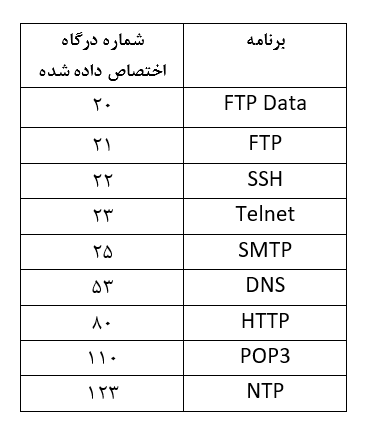
\includegraphics[width=0.5\textwidth]{ports.PNG}}
\end{table}

اما امروزه برنامه‌های جدید بخصوص برنامه‌های نظیر به نظیر از روش‌های مختلف برای پنهان کردن خود استفاده می‌کنند. آنها از درگاه‌های پویا و یا درگاه‌های دیگر برنامه‌های
شناخته‌شده در اتصالاتشان استفاده می‌کنند. که این امر باعث کاهش دقت طبقه‌بندی این روش شده‌است.

\section{روش مبتنی پیلود  }
با بوجود آمدن برنامه های نظیر به نظیر این روش، جایگزین قبلی شد. در این روش محتوای بسته‌ها برای پیدا کردن امضای برنامه‌های شناخته شده جستجو می‌شود. در جدول 2 یک نمونه از این امضاها که توسط کاراگیانیس\LTRfootnote{Thomas Karagiannis} استفاده شده است را می‌بینیم.

\begin{table}[!h]
\caption[نمونه امضاهای موجود در بسته های برخی از برنامه های پرکاربرد]{نمونه امضاهای موجود در بسته های برخی از برنامه های پرکاربرد\cite{shafiq2016network}}
\centerline{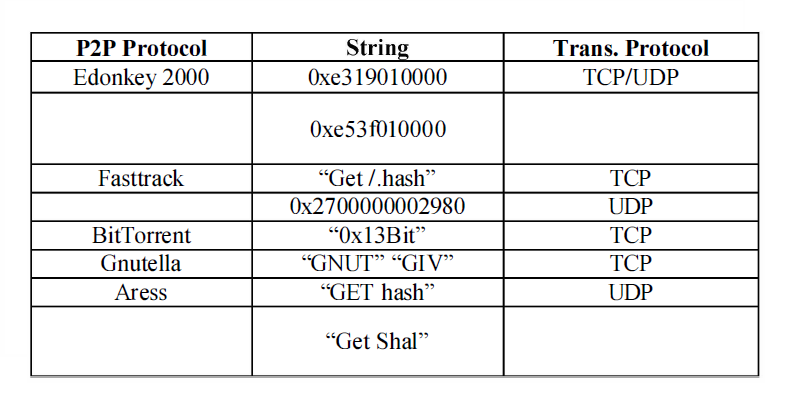
\includegraphics[width=0.9\textwidth]{signature.PNG}}
\end{table}

این روش به نسبت روش قبل دقیق تر عمل می‌کند اما چند مشکل دارد. مهم تر از همه این که نمی توان آن را بر روی بسته های رمزگذاری شده اعمال کرد. به علاوه تجزیه و تحلیل مستقیم داده ها باعث نقض حریم خصوصی کاربران می‌شود. همچنین این روش چون محتویات تمام بسته ها را بررسی میکند، نیازمند سیستم پردازشی به مراتب قوی تری نسبت به روش های دیگر است.

\section{روش مبتنی بر رفتار میزبان  }
ایده ی اصلی این روش این است که برنامه های مختلف الگوهای اتصال متفاوتی دارند. روش مبتنی بر رفتار میزبان، ارتباطات میان میزبان های خاص در یک شبکه را شناسایی میکند و الگوی ارتباط یک میزبان خاص با الگوی رفتار فعالیت های متفاوت مقایسه می‌شود. این روش پیلود بسته را برای طبقه بندی ترافیک استفاده نمی‌کند. پس می‌تواند بسته ها با محتوای رمزگذاری شده را نیز شناسایی کند.
\\
اما اشکال این روش این است که بیشتر تکنیک های مبتنی بر رفتار میزبان فرض می‌کند که میزبان های تحت نظارت در یک لحظه تنها از یک برنامه استفاده می‌کنند اما می‌دانیم در واقعیت، این وضعیت ممکن است هرگز اتفاق نیفتد. بیشتر کاربران از برنامه های زیادی به طور همزمان استفاده می‌کنند.
مشکل دیکری که در این روش بوجود میاد این است که برخی الگوهای رفتاری برنامه را نمی‌توان به آسانی کشف کرد. به مقدار حافظه و جریان های زیادی برای همه میزبان ها نیاز دارد تا بتواند الگوی اتصال را کشف کند. \cite{jangal}

\section{روش مبتنی بر یادگیری ماشین  }
یادگیری ماشین مجموعه ای از تکنیک‌ها برای داده کاوی و کشف دانش است که الگوهای ساختاری مفید در داده ها را جستجو میکند. این روش طبقه بندی مبتنی بر مجموعه داده های برچسب گذاری شده است. در این روش، یک طبقه بندی کننده یادگیری ماشین به عنوان ورودی آموزش داده می‌شود و سپس با استفاده از نمونه آموزش دیده، داده های ناشناخته طبقه بندی می‌شود.
دو روش اصلی در یادگیری ماشین وجود دارد. که در ادامه به بررسی هرکدام می‌پردازیم.

\subsection{یادگیری نظارت شده}
روش های یادگیری با نظارت، مبتنی بر دانش از پیش تعریف شده هستند. این الگوریتم ها در مرحله آموزش، نمونه های از پیش طبقه بندی شده (متشکل از ویژگی ها و
برچسب مرتبط با آنها) را به عنوان ورودی می‌گیرند و قوانین طبقه بندی ایجاد می‌شود. در مرحله طبقه بندی تلاش می‌کنند تا برچسب نمونه‌های بدون برچسب را پیشبینی
کنند.

\subsection{یادگیری بدون نظارت}
روش های یادگیری بدون نظارت، در مرحله یادگیری خود به هیچ دانش از قبل تعیین شده ای نیاز ندارند. این روش گروه های طبیعی را در داده ها کشف می‌کنند و روی کشف الگوهای موجود در داده ها تمرکز دارند. نمونه ها را بر اساس میزان شباهت ویژگی‌های آنها که توسط یک رویکرد اندازه گیری فاصله تعریف می‌شود. بنابر این در خروجی نمی‌توانیم نوع داده را به طور دقیق مشخص کنیم. صرفا داده های مشابه با هم در یک دسته قرار می‌گیرند.
\section{خلاصه}
در این فصل روش های کلی موجود برای طبقه بندی ترافیک شبکه از ابتدا تا کنون مورد بررسی قرار گرفت و راجع به مزایا و معیاب هر کدام بحث شد. روش مبتنی بر درگاه در برنامه های نظیر به نظیر دقت بالایی ندارد. روش مبتنی بر پیلود نیازمند سیستم پردازشی قوی می‌باشد و در شناسایی بسته های رمزگاری شده عاجز است. روش مبتنی بر رفتار میزبان صرفا برای زمان هایی که میزبان تنها از یک برنامه در لحظه استفاده می‌کند نتایج دقیقی تولید می‌کند. سپس روش های مبتنی بر یادگیری ماشین و انواع آن معرفی شد.
در ادامه روش مدل سازی و استفاده از یادگیری ماشین در طبقه بندی ترافیک شبکه توضیح داده می‌شود.. و سپس چند مورد از الگوریتم های معروف یادگیری ماشین و نیز پژوهش های انجام شده حول این موضوع بررسی می‌شود.
\chapter{مدل سازی روش یادگیری ماشین}
در این بخش مدل سازی و پیاده سازی انجام طبقه بندی ترافیک با استفاده از یادگیری ماشین در پنج مرحله بررسی می‌شود. شکل زیر خلاصه ای از این مراحل را نشان می‌دهد.

\begin{figure}[!h]
\centerline{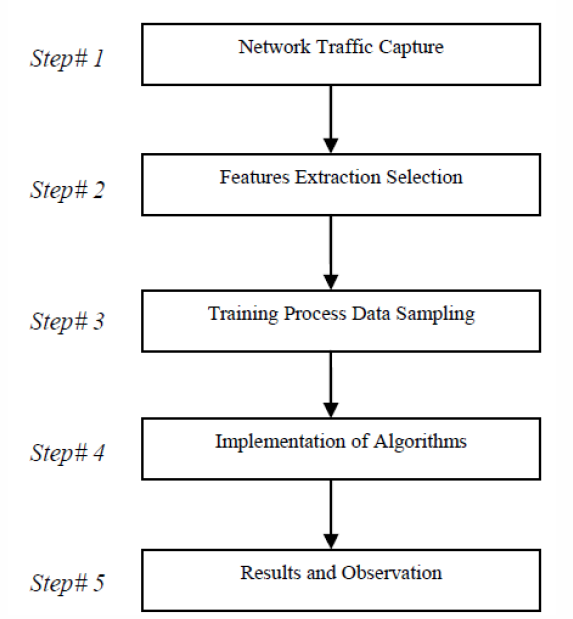
\includegraphics[width=0.6\textwidth]{steps.PNG}}
\caption[مدل پنج مرحله ای طبقه بندی ترافیک]{مدل پنج مرحله ای طبقه بندی ترافیک\cite{shafiq2016network}}
\end{figure}

همانطور که مشاهده می‌شود این پنج مرحله شامل جمع آوری داده، استخراج ویژگی ها، یادگیری نمونه، پیاده سازی الگوریتم و تحلیل نتایج می‌باشد، که در ادامه هر مرحله به اختصار توضیح داده می‌شود.

\section{جمع آوری داده}
اولین و مهم ترین بخش، جمع آوری داده یا به اصلاح گرفتن بسته\LTRfootnote{packet capture} های شبکه می باشد. ابزار های مختلفی برای این کار وجود دارد. از جمله معروف ترین ابزار ها در این زمینه وایرشارک\LTRfootnote{Wireshark} و تی سی پی دامپ\LTRfootnote{tcpdump} هستند که در پژوهش های مختلف از هر کدام از این ابزار ها استفاده شده است.

\section{استخراج ویژگی ها}
این مرحله که در پژوهش های مختلف غالبا با ابزارهای نت میت\LTRfootnote{Netmate} و پرل اسکریپت\LTRfootnote{Perl script} انجام می‌گیرد، ویژگی های خاصی از بسته ها استخراج می‌شود و با کمک آن ها دسته بند یادگیری ماشین\LTRfootnote{machine learning classifier} را آموزش می‌دهند. از جمله ویژگی های قابل استخراج می‌توان تعداد بسته ها، طول هر بسته، درگاه و پروتکل\LTRfootnote{protocol} مورد استفاده و غیره را نام برد. 

\section{یادگیری نمونه}
در مرحله ی سوم لازم است تا از داده های مورد نظر که در بخش اول بدست آمده، نمونه گیری انجام شود. از طرفی چون در این پژوهش از الگوریتم های یادگیری نظارت شده استفاده شده است، بر روی داده های دریافتی برچسب گذاری نیز انجام می‌شود تا بتوان به کمک آنها، بسته های ناشناخته را طبقه بندی کرد.

\section{پیاده سازی الگوریتم}
در این مرحله باید الگوریتم یادگیری ماشین مورد نظر بر روی داده های آموزش داده شده اعمال و پیاده سازی شوند. پژوهشگران معمولا به کمک ابزار وکا\LTRfootnote{Weka classification simulation tools}  این کار را انجام می‌دهند.


\section{بررسی و تحلیل نتایج}
در نهایت در بخش آخر ابراز وکا فرآیند تست روی داده ها را انجام می‌دهد و دقت ارزیابی انجام شده برای الگوریتم های مختلف را برای ما مشخص می‌کند.
با بررسی پژوهش های انجام شده بر روی شش الگوریتم یادگیری ماشین درخت تصمیم آر بی اف\LTRfootnote{RBF decision tree}، ماشین بردار پشتیبان\LTRfootnote{support vector machine (SVM)}، \lr{C4.5}، نزدیک ترین همسایه\LTRfootnote{nearest neighbor}، نیوبیز\LTRfootnote{naive bayes}، و شبکه بیز\LTRfootnote{bayesian network} نتایج زیر حاصل شده است. \cite{shafiq2016network, jamuna2013efficient}

\begin{table}[!h]
\caption{دقت طبقه بندی الگوریتم های مختلف یادگیری ماشین}
\centerline{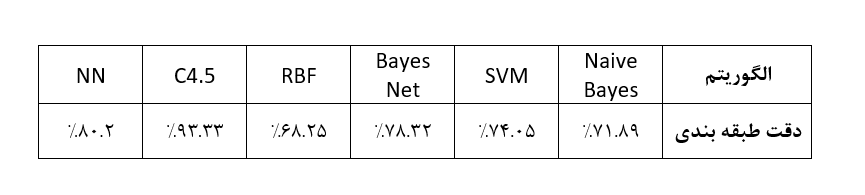
\includegraphics[width=1\textwidth]{accuracy.PNG}}
\end{table}

همانطور که در جدول نشان داده شده است، از بین الگوریتم های مورد استفاده در این پژوهش، با استفاده از الگوریتم یادگیری ماشین \lr{C4.5} توانسته ایم به دقت بیش از 93 درصد برای طبقه بندی ترافیک شبکه دست پیدا کنیم. الگوریتم نزدیک ترین همسایه نیز دقت تقریبا 80 درصدی را نشان می‌دهد. پس از آن برای الگوریتم های شبکه بیز، ماشین بردار پشتیبان و نیو بیز نیز دقتی بین 70 تا 80 درصد بدست آمده است.


\section{خلاصه}

در این بخش قدم به قدم با مراحل مدل سازی و پیاده سازی روش یادگیری ماشین آشنا شدیم و مشاهده کردیم که الگوریتم یادگیری ماشین \lr{C4.5} با دقتی معادل 5.93 درصد، بسته های شبکه را به درستی طبقه بندی می‌کند.
\chapter{ نتیجه گیری و پیشنهادها}
\section{نتیجه گیری}

شناسایی جریان جاری روی ترافیک اینترنت روی جنبه های مختلف شبکه مانند امنیت تأثیر زیادی دارد. همچنین تشخیص جریان های ترافیک باعث برنامه ریزی صحیح در قسمت های مختلف شبکه مانند تخصیص منابع، بهبود کیفیت خدمات سرویس و غیره می شود. بنابراین، با توجه به اهمیت شناسایی جریان های ترافیک اینترنت، در این پژوهش انواع روش های موجود برای طبقه بندی ترافیک که از گذشته تا کنون استفاده می‌شده است، مورد بررسی قرار گرفت و در مورد مزایا و معایب هرکدام بحث شد. در ادامه آزمایش های انجام شده برای شش مورد از الگوریتم های یادگیری ماشین برای طبقه بندی ترافیک شبکه با یکدیگر مقایسه شد که دیدیم الگوریتم \lr{C4.5} با دقت بیشتری نسبت به سایر الگوریتم ها این کار را انجام می دهد.

\section{پیشنهادها}
امروزه با گسترش علم یادگیری ماشین همچنان می توان امیدوار بود که با بهبود هر کدام از الگوریتم های موجود بتوان به دقت بسیار بیشتری نسبت به آنچه تا کنون بدست آمده برسیم. امید است با مطالعه ی بیشتر بر روی الگوریتم های یادگیری ماشین و ترکیب یا بهبود روش های موجود به دقت بالاتری در طبقه بندی ترافیک و درنتیجه امنیت و کیفیت بالاتری برای شبکه ی اینترنت برسیم.
%--------------------------------------------------------------------------appendix( مراجع و پیوست ها)
\chapterfont{\vspace*{-2em}\centering\LARGE}%

\appendix
\bibliographystyle{plain-fa}
\bibliography{references}
%\chapter*{‌پیوست}
\markboth{پیوست}{}
\addcontentsline{toc}{chapter}{پیوست}
موضوعات مرتبط با متن گزارش پایان نامه كه در يكی از گروه‌های زير قرار می‌گيرد، در بخش پيوست‌ها آورده شوند:
\begin{enumerate}
\item  اثبات های رياضی يا عمليات رياضی طولانی‌.‌
\item داده و اطلاعات نمونه (های) مورد مطالعه (\lr{Case Study}) چنانچه طولانی باشد‌.‌
\item نتايج كارهای ديگران چنانچه نياز به تفصيل باشد‌.‌
\item مجموعه تعاريف متغيرها و پارامترها، چنانچه طولانی بوده و در متن به انجام نرسيده باشد‌.‌
\end{enumerate}
% براي شماره‌گذاري روابط، جداول و اشكال موجود در پيوست‌ از ساختار متفاوتي نسبت به متن اصلي استفاده مي‌شود كه در زير به‌عنوان نمونه نمايش داده شده‌است. 
% \begin{equation}
%F=ma
%\end{equation}
\section*{کد میپل }
\begin{latin}
\begin{verbatim}

with(DifferentialGeometry):
with(Tensor):
DGsetup([x, y, z], M)
																	frame name: M
a := evalDG(D_x)
																	D_x
b := evalDG(-2 y z D_x+2 x D_y/z^3-D_z/z^2)


\end{verbatim}
\end{latin}
%--------------------------------------------------------------------------dictionary(واژه نامه ها)
%اگر مایل به داشتن صفحه واژه‌نامه نیستید، خط زیر را غیر فعال کنید.
\parindent=0pt
%%
\chapter*{واژه‌نامه‌ی فارسی به انگلیسی}
\pagestyle{style9}

\addcontentsline{toc}{chapter}{واژه‌نامه‌ی فارسی به انگلیسی}
%%%%%%
\begin{multicols*}{2}

{\bf آ}
\vspace*{3mm}


\farsiTOenglish{اسکالر}{Scalar}


\vspace*{3mm}
{\bf ب}
\vspace*{3mm}

\farsiTOenglish{بالابر}{Lift}


\vspace*{3mm}
{\bf پ}
%%\vspace*{3mm}

\farsiTOenglish{پایا}{Invariant}



\vspace*{3mm}
{\bf ت}
%%\vspace*{3mm}

\farsiTOenglish{ تناظر }{Correspondence}


\vspace*{3mm}
{\bf ث}
%%\vspace*{3mm}

\farsiTOenglish{ثابت‌ساز}{Stabilizer}

\vspace*{3mm}
{\bf ج}
%%\vspace*{3mm}

\farsiTOenglish{جایگشت}{Permutation}



\vspace*{3mm}
{\bf چ}
%%\vspace*{3mm}


\farsiTOenglish{چند جمله‌ای }{Polynomial}

\vspace*{3mm}
{\bf ح}
%%\vspace*{3mm}

\farsiTOenglish{حاصل‌ضرب دکارتی}{Cartesian product}


\vspace*{3mm}
{\bf خ}
%%\vspace*{3mm}

\farsiTOenglish{خودریختی}{Automorphism}

\vspace*{3mm}
{\bf د}
%%\vspace*{3mm}

\farsiTOenglish{درجه}{Degree}


\vspace*{3mm}
{\bf ر}
%%\vspace*{3mm}


\farsiTOenglish{ریزپردازنده}{microprocessor}


\vspace*{3mm}
{\bf ز}
%%\vspace*{3mm}


\farsiTOenglish{زیرمدول}{Submodule}


\vspace*{3mm}
{\bf س}
%%\vspace*{3mm}

\farsiTOenglish{سرشت}{Character}


\vspace*{3mm}
{\bf ص}
%%\vspace*{3mm}

\farsiTOenglish{صادقانه}{Faithful}

\vspace*{3mm}
{\bf ض}
%%\vspace*{3mm}

\farsiTOenglish{ضرب داخلی}{Inner product}

\vspace*{3mm}
{\bf ط}
%%\vspace*{3mm}


\farsiTOenglish{طوقه}{Loop}


\vspace*{3mm}
{\bf ظ}
%%\vspace*{3mm}


\farsiTOenglish{ظرفیت}{Valency}
 
\vspace*{3mm}
{\bf ع}
%%\vspace*{3mm}


\farsiTOenglish{عدم مجاورت}{Nonadjacency}



\vspace*{3mm}
{\bf ف}
%%\vspace*{3mm}

\farsiTOenglish{فضای برداری}{Vector space}



\vspace*{3mm}
{\bf ک}
%%\vspace*{3mm}

\farsiTOenglish{کاملاً تحویل‌پذیر}{Complete reducibility}


\vspace*{3mm}
{\bf گ}
%%\vspace*{3mm}


\farsiTOenglish{گراف}{Graph}



\vspace*{3mm}
{\bf م}
%%\vspace*{3mm}

\farsiTOenglish{ماتریس جایگشتی}{Permutation matrix }


\vspace*{3mm}
{\bf ن}
%%\vspace*{3mm}

\farsiTOenglish{ناهمبند}{Disconnected}


\vspace*{3mm}
{\bf و}
%%\vspace*{3mm}

\farsiTOenglish{وارون‌پذیر}{Invertible}


\vspace*{3mm}
{\bf ه}
%%\vspace*{3mm}

\farsiTOenglish{همبند}{Connected}



\vspace*{3mm}
{\bf ی}
%%\vspace*{3mm}

\farsiTOenglish{یال}{Edge}




\end{multicols*}%
%%%%%%%
\chapter*{ واژه‌نامه‌ی انگلیسی به فارسی}
\pagestyle{style9}
\lhead{\thepage}\rhead{واژه‌نامه‌ی انگلیسی به فارسی}
\addcontentsline{toc}{chapter}{واژه‌نامه‌ی انگلیسی به فارسی}

\LTRmulticolcolumns
\begin{multicols}{2}
{\hfill\bf  \lr{A}}
%%\vspace*{1.5mm}

\englishTOfarsi{Automorphism}{خودریختی}

\vspace*{3mm}
{\hfill\bf   \lr{B}}
%%\vspace*{1.5mm}

\englishTOfarsi{Bijection}{دوسویی}

\vspace*{3mm}
{\hfill\bf   \lr{C}}
%%\vspace*{1.5mm}

\englishTOfarsi{Cycle group}{گروه دوری}

\vspace*{3mm}
{\hfill\bf   \lr{D}}
%%\vspace*{1.5mm}

\englishTOfarsi{Degree}{درجه}

\vspace*{3mm}
{\hfill\bf   \lr{E}}
%%\vspace*{1.5mm}

\englishTOfarsi{Edge}{یال}

\vspace*{3mm}
{\hfill\bf   \lr{F}}
%%\vspace*{1.5mm}

\englishTOfarsi{Function}{تابع}

\vspace*{3mm}
{\hfill\bf   \lr{G}}
%%\vspace*{1.5mm}

\englishTOfarsi{Group}{گروه}

\vspace*{3mm}
{\hfill\bf   \lr{H}}
%%\vspace*{1.5mm}

\englishTOfarsi{Homomorphism}{همریختی}

\vspace*{3mm}
{\hfill\bf   \lr{I}}
%%\vspace*{1.5mm}

\englishTOfarsi{Invariant}{پایا}

\vspace*{3mm}
{\hfill\bf   \lr{L}}
%%\vspace*{1.5mm}

\englishTOfarsi{Lift}{بالابر}

\vspace*{3mm}
{\hfill\bf   \lr{M}}
%%\vspace*{1.5mm}

\englishTOfarsi{Module}{مدول}

\vspace*{3mm}
{\hfill\bf   \lr{N}}
%%\vspace*{1.5mm}

\englishTOfarsi{Natural map}{نگاشت طبیعی}

\vspace*{3mm}
{\hfill\bf   \lr{O}}
%%\vspace*{1.5mm}

\englishTOfarsi{One to One}{یک به یک}

\vspace*{3mm}
{\hfill\bf   \lr{P}}
%%\vspace*{1.5mm}

\englishTOfarsi{Permutation group}{گروه جایگشتی}

\vspace*{3mm}
{\hfill\bf   \lr{Q}}
%%\vspace*{1.5mm}

\englishTOfarsi{Quotient graph}{گراف خارج‌قسمتی}

 \vspace*{3mm}
{\hfill\bf   \lr{R}}
%%\vspace*{1.5mm}

\englishTOfarsi{Reducible}{تحویل پذیر}

\vspace*{3mm}
{\hfill\bf   \lr{S}}
%%\vspace*{1.5mm}

\englishTOfarsi{Sequence}{دنباله}

 \vspace*{3mm}
{\hfill\bf   \lr{T}}
%%\vspace*{1.5mm}

\englishTOfarsi{Trivial character}{سرشت بدیهی}

\vspace*{3mm}
{\hfill\bf   \lr{U}}
%%\vspace*{1.5mm}

\englishTOfarsi{Unique}{منحصربفرد}

\vspace*{3mm}
{\hfill\bf   \lr{V}}
%%\vspace*{1.5mm}

\englishTOfarsi{Vector space}{فضای برداری}
\end{multicols}
%--------------------------------------------------------------------------index(نمایه)
%اگر مایل به داشتن صفحه نمایه نیستید، خط زیر را غیر فعال کنید.
\pagestyle{style7}
\printindex
\pagestyle{style7}
%%کلمات کلیدی انگلیسی
\latinkeywords{Write a 3 to 5 KeyWords is essential. Example: AUT, M.Sc., Ph. D,..}
%چکیده انگلیسی

\en-abstract{
This page is accurate translation from Persian abstract into English.
}
%%%%%%%%%%%%%%%%%%%%% کدهای زیر را تغییر ندهید.

\newpage
\thispagestyle{empty}
\begin{latin}
\section*{\LARGE\centering Abstract}

\een-abstract

\vspace*{.5cm}
{\large\textbf{Key Words:}}\par
\vspace*{.5cm}
\elatinkeywords
\end{latin}
%% در این فایل، عنوان پایان‌نامه، مشخصات خود و چکیده پایان‌نامه را به انگلیسی، وارد کنید.
%%%%%%%%%%%%%%%%%%%%%%%%%%%%%%%%%%%%
\baselineskip=.6cm
\begin{latin}

\latinfaculty{Department of Computer Engineering}


\latintitle{Network Traffic Classification Using Machine Learning Algorithms}


\firstlatinsupervisor{Dr.Safabakhsh}

%\secondlatinsupervisor{Second Supervisor}

%\firstlatinadvisor{Dr. }

%\secondlatinadvisor{Second Advisor}

\latinname{Mohammad Mahdi}

\latinsurname{Hejrati}

\latinthesisdate{May \& 2021}

\latinvtitle
\end{latin}

\end{document}